\subsection{Peripherie}

\subsubsection{Maschinengestell}
\label{maschinengestell}
\begin{wrapfigure}[16]{r}{6cm}
	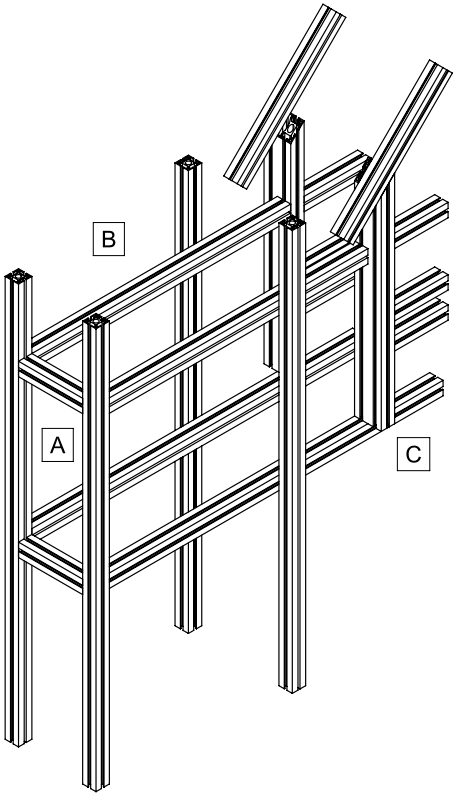
\includegraphics[scale=0.41]{Illustrationen/6-Umsetzung/maschinengestell.PNG}
	\caption{Maschinengestell}
	\label{fig:maschinengestell}
\end{wrapfigure}

\textit{(ygu)} Das Maschinengestell basiert auf dem Baukasten System von Kanya AG. Die Profile von Kanya AG eignen sich aus folgenden Gründen:
\begin{itemize}
	\item Dieses System ist einfach im Aufbau und der Montage. Das Maschinengestell ist so aufgebaut, dass eine Anpassung der Höhe (Punkt B in Abbildung \ref{fig:maschinengestell}) und die überstehende Länge der Setzeinheit (C) möglich ist. Diese Flexibilität wird durch die Verwendung der Universallverbinder von Kanya AG möglich.
	
	\item Das Profil hat an jeder Seite eine Längsnut. Dies bietet eine simple Lösung zur Montage der Montagebleche der Setzeinheit sowie Vereinzelung. Zudem ist im hinteren Teil des Gestells (A) eine Aluminiumplatte zur Montage der Elektronik vorgesehen.
	
	\item Die Tatsache, dass die Hochschule Luzern bei Kanya AG bereits Kunde ist, hebt Kanya AG von anderen Konkurrenten ab. Die positiven Erfahrungen und raschen Lieferzeiten überzeugen.
\end{itemize}
Weitere Informationen zum Baukastensystem von Kanya AG ist aus dem Katalog zu entnehmen \cite{kanya}.
\subsubsection{Verdrahtung}